\notechapter{N-20211007}{From Diophantine Inequalities to Arithmetic Deformation}

\section{The question is an inequality, not a slogan}

Fesenko's survey presents inter-universal Teichmueller theory under another name: arithmetic deformation theory.  This name is useful because it puts the reader's attention on the mathematical target before the new language appears.  The target is not first of all a mystical ``inter-universal'' philosophy.  It is a family of Diophantine inequalities in which one wants to control the arithmetic size of a curve, an elliptic curve, or a rational point.

The basic shape is always the same.  One side measures size: height, discriminant, or a quantity built out of bad reduction.  The other side measures the places where the object is allowed to be complicated: conductor, ramification, different, or a divisor of excluded points.  The problem is to prove that the first kind of size cannot grow too fast compared with the second kind of size.

\begin{definition}[Number field and absolute Galois group]
A number field is a finite extension \(K/\mathbb Q\).  If \(K^{\mathrm{alg}}\) is an algebraic closure of \(K\), its absolute Galois group is
\[
  G_K=\operatorname{Gal}(K^{\mathrm{alg}}/K),
\]
regarded as a profinite topological group.
\end{definition}

The appearance of \(G_K\) is not decoration.  A large part of the story leading to IUT asks how much arithmetic geometry can be recovered from groups of symmetries.  In ordinary algebraic geometry one starts with equations and then studies automorphisms or fundamental groups.  Anabelian geometry tries to reverse this direction: from a suitable fundamental group, recover the geometric or arithmetic object.

\section{A first chain of rigidity results}

The first rigidity theorem in this note is about number fields alone.

\begin{theorem}[Neukirch--Ikeda--Uchida, schematic form]
Let \(K_1\) and \(K_2\) be number fields.  An isomorphism of topological groups
\[
  G_{K_1}\cong G_{K_2}
\]
comes from a unique field-theoretic identification of the corresponding algebraic closures, in a way compatible with the two number fields.  Thus, for number fields, the absolute Galois group remembers the field.
\end{theorem}

This theorem should be read as a warning against the naive view that a Galois group is only an auxiliary invariant.  In the number-field case, the group is so rigid that the field can be reconstructed from it.

The next theorem connects curves with a surprisingly small amount of ramification.

\begin{theorem}[Belyi]
Let \(C\) be an irreducible smooth projective algebraic curve over a field of characteristic zero.  Then \(C\) can be defined over \(\overline{\mathbb Q}\) if and only if there exists a finite morphism
\[
  C\longrightarrow \mathbb P^1
\]
which is ramified over at most three points of \(\mathbb P^1\).
\end{theorem}

Such maps are called Belyi maps.  For this note, the important point is not the proof but the direction of thought.  Curves over number fields, coverings of \(\mathbb P^1\setminus\{0,1,\infty\}\), and Galois/fundamental-group data are not separate topics.  They are different faces of the same arithmetic geometry.

\begin{remark}[Why this belongs in the IUT entrance]
Fesenko emphasizes that versions of Belyi maps are used later in arithmetic deformation theory and its application to Diophantine geometry.  This is why the story does not begin directly with theta-links.  Before one reaches theta-links, one has already entered a world where curves, number fields, and fundamental groups are designed to remember one another.
\end{remark}

\section{From Mordell finiteness to effective inequalities}

Faltings' theorem gives a finiteness result.

\begin{theorem}[Faltings--Mordell]
If \(C\) is a smooth projective curve of genus \(>1\) over a number field \(K\), then \(C(K)\) is finite.
\end{theorem}

Finiteness is a qualitative statement.  The effective Mordell problem asks for more: not only that rational points are finite, but that their heights can be bounded in terms of computable arithmetic data.  In the background of Fesenko's survey, this effective direction sits beside several closely related conjectures:
\[
  \text{effective Mordell},\qquad
  \text{Szpiro},\qquad
  abc,\qquad
  \text{Frey},\qquad
  \text{Vojta for hyperbolic curves}.
\]
These are not identical statements, but Fesenko presents them as a closely connected cluster.  The important organizing idea is that they all seek an inequality strong enough to control Diophantine complexity.

\section{The Szpiro inequality as a concrete target}

The Szpiro conjecture is a good first model because it is phrased directly in terms of elliptic curves and bad reduction.  Let \(E_K\) be an elliptic curve over a number field \(K\).  In the split multiplicative situation, the bad fibers of the minimal regular proper model have type \(I_{n_v}\).  Here \(v\) runs over nonarchimedean valuations of \(K\), \(k(v)\) is the residue field, and \(n_v\) is the number of components in the bad fiber.

\begin{definition}[Conductor-size and discriminant-size, split multiplicative model]
In the split multiplicative case, the logarithmic discriminant-size and conductor-size are, schematically,
\[
  \sum_{v\ \mathrm{bad}} n_v\log |k(v)|,
  \qquad
  \sum_{v\ \mathrm{bad}} \log |k(v)|.
\]
The first expression counts bad fibers with multiplicity \(n_v\).  The second remembers only the bad places themselves.
\end{definition}

The conjectural Szpiro inequality then has the form
\[
  \sum_{v\ \mathrm{bad}} n_v\log |k(v)|
  \leq
  c+(6+\epsilon)\sum_{v\ \mathrm{bad}}\log |k(v)|,
\]
for every \(\epsilon>0\), with a constant \(c\) depending on \(K\) and \(\epsilon\).  Equivalently, using the absolute norms of the minimal discriminant and the conductor, one writes
\[
  N(\operatorname{Disc}E_K)
  \leq
  c' N(\operatorname{Cond}E_K)^{6+\epsilon}.
\]

\begin{remark}[The meaning of the exponent]
The number \(6\) is not a random constant inserted into the conjecture.  In Fesenko's discussion it is connected with the geometric Szpiro-type inequality for elliptic surfaces and with the comparison between the arithmetic and geometric sides of the problem.  For the present note, the safe takeaway is that Szpiro is an inequality bounding discriminant-size by conductor-size.
\end{remark}

A very simple reading is this: the conductor records where the elliptic curve behaves badly; the discriminant records how badly it behaves there.  Szpiro predicts that ``how badly'' cannot be much larger than a fixed power of ``where badly''.

\section{Vojta's inequality and the hyperbolic curve viewpoint}

The Vojta form is closer to the geometry of punctured curves.

\begin{definition}[Hyperbolic curve]
Over a field of characteristic zero, a hyperbolic curve is a smooth projective geometrically connected curve of genus \(g\) with \(r\) points removed, such that
\[
  2-2g-r<0.
\]
Examples include \(\mathbb P^1\setminus\{0,1,\infty\}\) and an elliptic curve with the origin removed.
\end{definition}

The condition is not merely topological decoration.  Hyperbolic curves have nonabelian algebraic fundamental groups, and these groups are the kind of objects anabelian geometry can hope to use for reconstruction.

Let \(C\) be a smooth proper geometrically connected curve over a number field \(K\), and let \(D\) be a reduced effective divisor on \(C\) such that \(C\setminus D\) is hyperbolic.  Vojta-type inequalities compare a height attached to \(\omega_C(D)\) with terms measuring ramification and contact with \(D\):
\[
  h_{\omega_C(D)}(x)
  \leq
  c+(1+\epsilon)
  \bigl(\log\operatorname{-diff}_C(x)+\log\operatorname{-cond}_D(x)\bigr).
\]
Here \(\log\operatorname{-diff}\) measures the arithmetic complexity of the field of definition of \(x\), while \(\log\operatorname{-cond}\) measures intersection with the divisor \(D\).

\begin{remark}[Why Belyi maps reappear]
Fesenko notes that Belyi maps reduce the Vojta conjecture for such \((C,D)\) to the special case
\[
  C=\mathbb P^1,\qquad D=[0]+[1]+[\infty].
\]
Thus the same three-punctured projective line that appears in Belyi's theorem also acts as a universal testing ground for the Diophantine inequality.
\end{remark}

\section{Arithmetic fundamental groups}

For a geometrically integral scheme \(X\) over a perfect field \(K\), there is a fundamental exact sequence
\[
  1\longrightarrow \pi_1^{\mathrm{geom}}(X)
  \longrightarrow \pi_1(X)
  \longrightarrow G_K
  \longrightarrow 1,
\]
where
\[
  \pi_1^{\mathrm{geom}}(X)=\pi_1(X\times_K K^{\mathrm{alg}}).
\]
For schemes over number fields or related fields, \(\pi_1(X)\) is often called an arithmetic fundamental group.

\begin{definition}[Anabelian reconstruction, guiding form]
Anabelian reconstruction is the idea that, for suitable schemes \(X\), one can recover the arithmetic or geometric object from its algebraic fundamental group together with the projection
\[
  \pi_1(X)\longrightarrow G_K.
\]
The slogan is not that every space is determined by its fundamental group, but that certain highly nonabelian arithmetic schemes are rigid enough for this to happen.
\end{definition}

In the IUT entrance, this matters because the later theory needs structures that survive when ordinary ring-theoretic comparison is no longer available.  Fesenko summarizes the transition as follows: arithmetic deformation theory is related to anabelian geometry, but uses a different package of tools, including mono-anabelian geometry, nonarchimedean theta-functions, monoid-theoretic categories, and deconstruction/reconstruction of ring structures.

\section{The local elliptic curve model: Tate curves and q-parameters}

The first truly arithmetic-deformation object in the survey is not the \(abc\) equation itself.  It is an elliptic curve with split multiplicative reduction and its local \(q\)-parameters.

Let \(E_F\) be an elliptic curve over a number field \(F\).  Suppose that, at a bad nonarchimedean valuation \(v\), the curve has split multiplicative reduction.  Let \(F_v\) be the completion of \(F\) at \(v\).  Then locally one has a Tate uniformization
\[
  E_F(F_v)\cong F_v^{\times}/\langle q_v\rangle,
\]
where \(q_v\in F_v^{\times}\) is the local \(q\)-parameter and \(\langle q_v\rangle\) is the cyclic subgroup generated by \(q_v\).

\begin{definition}[The idele \(q_{E_F}\)]
Define an idele \(q_{E_F}\in \mathbb A_F^{\times}\) by setting its component to be
\[
  (q_{E_F})_v=\begin{cases}
  q_v,& v\text{ a bad split multiplicative valuation},\\
  1,& v\text{ archimedean or good reduction}.
  \end{cases}
\]

after choosing the local \(q_v\) at each bad valuation.
\end{definition}

The valuation of \(q_v\) records the number \(n_v\) of components of the corresponding bad fiber.  Therefore the degree of this idele is not an artificial invariant: it packages the left-hand side of the Szpiro inequality.

\section{Normalised degree as log-volume}

Fesenko uses ideles to define a normalised degree.  Let \(k\) be a number field and \(\mathbb A_k^{\times}\) its idele group.  For \(\alpha\in\mathbb A_k^{\times}\), the non-normalised degree is
\[
  \deg_k(\alpha)=-\log |\alpha|,
\]
where \(|\alpha|\) is the module by which multiplication by \(\alpha\) scales Haar measure on the adele ring.  The normalised degree is
\[
  \deg(\alpha)=\frac{1}{[k:\mathbb Q]}\deg_k(\alpha).
\]
This normalisation is stable under finite field extension, which is why the same symbol \(\deg\) can be used after passing to larger number fields.

\begin{remark}[Why log-volume enters]
Because of the minus sign, \(-\deg(\alpha)\) is naturally interpreted as a log-volume.  In the later IUT inequality, the left side is written in terms of \(-\deg q_E\).  This is why the problem of bounding Szpiro-type data becomes a problem about bounding log-volumes.
\end{remark}

For the elliptic curve above, Fesenko identifies the goal as giving a suitable upper bound on
\[
  \deg q_{E_F}.
\]
This is the cleanest first target of arithmetic deformation theory in the survey.

\section{Why ordinary scheme-theoretic geometry is not enough}

The next move is the point where the theory stops looking like ordinary algebraic geometry.  Fix a prime \(l>3\), relatively prime to the bad valuations and to the relevant local valuation numbers.  For a bad valuation \(v\), Fesenko records a monoid-theoretic transformation on the submonoid of \(F_v^{\times}\) generated by units and \(q_v\):
\[
  q_v\longmapsto q_v^{m^2},
  \qquad
  u\longmapsto u\quad (u\in\mathcal O_{F_v}^{\times}),
\]
where
\[
  1\leq m\leq \frac{l-1}{2}.
\]
The element \(q_v^{m^2}\) is later viewed as a special value of a nonarchimedean theta-function.

\begin{proposition}[The first deformation warning]
The transformation
\[
  q_v\mapsto q_v^{m^2},\qquad u\mapsto u
\]
should be read as monoid-theoretic rather than ring-theoretic.  It is not a morphism of schemes and does not preserve the full ring structure.
\end{proposition}

\begin{proof}
The point is conceptual rather than computational.  A ring morphism must respect both multiplication and addition.  The displayed transformation is defined on multiplicative data: the local units and the generator \(q_v\) of the Tate period subgroup.  It is designed to manipulate multiplicative/theta data, not to preserve addition in \(F_v\).  Thus it belongs to the monoid-theoretic side of the theory.
\end{proof}

This is the first reason the word ``deformation'' is appropriate.  The ring structure is not transported intact.  It is partly dismantled so that certain multiplicative and theta-theoretic information can be moved, after which one needs reconstruction tools.

\section{The route from deformation to inequality}

The full theta-link belongs to later notes.  But the route can already be drawn.

\begin{center}
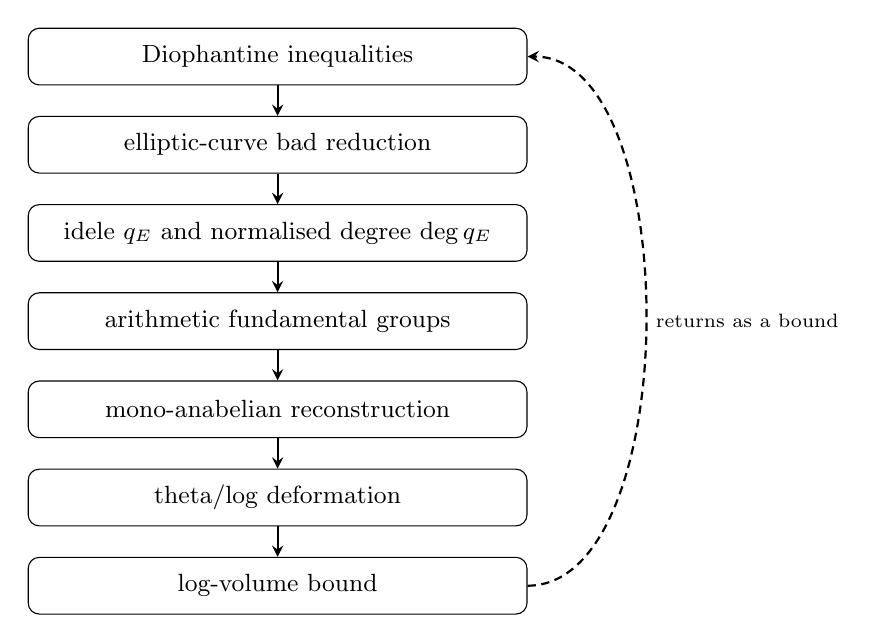
\begin{tikzpicture}[
  >=stealth,
  routebox/.style={draw,rounded corners,align=center,text width=6.1cm,minimum height=0.72cm,font=\small},
  route/.style={->,thick}
]
  \node[routebox] (A) at (0,0) {Diophantine inequalities};
  \node[routebox] (B) at (0,-1.12) {elliptic-curve bad reduction};
  \node[routebox] (C) at (0,-2.24) {idele \(q_E\) and normalised degree \(\deg q_E\)};
  \node[routebox] (D) at (0,-3.36) {arithmetic fundamental groups};
  \node[routebox] (E) at (0,-4.48) {mono-anabelian reconstruction};
  \node[routebox] (F) at (0,-5.60) {theta/log deformation};
  \node[routebox] (G) at (0,-6.72) {log-volume bound};

  \draw[route] (A) -- (B);
  \draw[route] (B) -- (C);
  \draw[route] (C) -- (D);
  \draw[route] (D) -- (E);
  \draw[route] (E) -- (F);
  \draw[route] (F) -- (G);
  \draw[route,densely dashed]
    (G.east) .. controls +(2.0,0) and +(2.0,0) ..
    node[right,font=\scriptsize,align=center] {returns as\ a bound}
    (A.east);
\end{tikzpicture}
\end{center}

The diagram is not a proof.  It is a navigation map.  Starting from Diophantine inequalities, one passes to elliptic curves and their bad reduction.  The bad reduction is encoded by \(q_E\).  IUT then introduces a deformation machine involving arithmetic fundamental groups, mono-anabelian reconstruction, theta-links, log-links, and log-theta-lattices.  The intended output is a log-volume inequality which returns to the original Diophantine problem.

\begin{theorem}[Main IUT inequality, schematic form]
In Fesenko's account, the main theorem of IUT gives a bound on log-volumes of the form
\[
  -\deg q_E\leq -\deg \Theta_E,
\]
where the right-hand side is the log-volume of a union of possible images of theta-data after applying the theta-link, subject to specified indeterminacies.
\end{theorem}

The statement above is deliberately schematic.  It records the mathematical role of the theorem, not the construction of the objects.  The important point for this first note is that the theorem does not directly say ``abc is true''.  It gives a bound on a deformation volume.  A further computation of the right-hand side is then used to obtain a bound of the desired Diophantine kind.

\begin{remark}[The bridge to later notes]
The words theta-link, log-link, log-theta-lattice, indeterminacy, and multiradiality all belong to the mechanism behind \(\Theta_E\).  They should not be treated as decorative terminology.  They are the devices by which the theory tries to compare arithmetic data after the ordinary ring structure has been deconstructed.
\end{remark}

\section{What the schematic comparison establishes}

The first entrance to IUT should therefore be remembered through four questions.

\begin{enumerate}
  \item What is being bounded?  The initial concrete target is \(\deg q_E\), which packages the bad-reduction side of a Szpiro-type inequality.
  \item What is rigid?  Absolute Galois groups and arithmetic fundamental groups can, in suitable settings, remember number fields or curves.
  \item What is allowed to vary?  The ordinary ring structure is no longer transported as a single indivisible object; multiplicative and additive aspects are separated.
  \item Why is advanced machinery needed?  Once ordinary scheme morphisms are not enough, one needs mono-anabelian reconstruction, Kummer-type methods, nonarchimedean theta-functions, and log-volume control.
\end{enumerate}

This is already a mathematical picture, but not yet the full theory.  The next note should begin where this one stops: with the moment when the map involving \(q_v^{m^2}\) becomes part of the theta-link, and when the lost additive structure has to be handled through log-links and log-shells.

